\documentclass[bigger, aspectratio=169]{beamer}

\usepackage{booktabs}
\usetheme{metropolis}
\metroset{block=fill}
\setbeamercolor{background canvas}{bg=white}
\usepackage[english]{babel}
\usepackage[utf8]{inputenc}
\usepackage{mathtools,amssymb,amsthm}
\usepackage{graphicx}
%\usepackage{tikz}
%\usetikzlibrary{calc}
\usepackage{xcolor}
\usepackage{color, colortbl}

\title{Experimental Evaluation of Similarity Measures for Educational Items}

\author{Jaroslav \v{C}ech\'ak \and Radek Pel\'anek\\[5mm]
%Masaryk University Brno\\
%Czech Republic
%\includegraphics[width=.35\linewidth]{figures/al-logo}\\[3mm]
}

\definecolor{gold}{HTML}{b27a01}
\definecolor{grass}{HTML}{419c03}

\newcommand{\img}[2]{
  \begin{center}
    \includegraphics[width=#1\linewidth]{figures/#2}
  \end{center}
}

\newcommand{\mute}[1]{
  {\color{gray}{#1}}
}

\date{\vfill EDM 2021\hfill \includegraphics[width=.35\linewidth]{figures/al-logo}}

\begin{document}

\frame{\titlepage}

\begin{frame}
	\frametitle{Problem}
	\centering
	\footnotesize
	\begin{tabular}{p{.28\linewidth}llp{.43\linewidth}}
		\toprule
		item stem & correct & distractor & explanation \\
		\midrule
		I \_ to the gym once a week. & go & am going & When talking about
		periodical events, we use present simple tense. \\
		He \_ breakfast every day. & eats & is eating & When talking about
		periodical events, we use present simple tense. \\
		I \_ this book. & like & am liking & When talking about general state, we use present simple tense. The 
		verb to like is not used in continuous form. \\
%		Take your umbrella, it \_. & is raining & rains & When talking about currently ongoing events, we use 
%		present continuous tense. \\
		\bottomrule
	\end{tabular}
	
	\bigskip
	
	54 knowledge components, 68 item sets, $4\,348$ items 
	
\end{frame}

\begin{frame}
	\frametitle{Solution}
	\begin{center}
		\includegraphics[width=0.65\linewidth]{figures/similarity_visualization}
	\end{center}
\end{frame}

\begin{frame}
	\frametitle{Solution}
	\begin{center}
		\includegraphics[width=0.65\linewidth]{figures/similarity_visualization_outlier}
	\end{center}
\end{frame}

\begin{frame}
	\frametitle{Solution}
	\begin{center}
		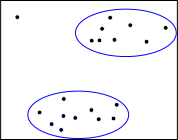
\includegraphics[width=0.65\linewidth]{figures/similarity_visualization_clusters}
	\end{center}
\end{frame}

\begin{frame}
	\frametitle{Solution}
	\begin{center}
		\includegraphics[width=0.65\linewidth]{figures/similarity_visualization_gap}
	\end{center}
\end{frame}

\begin{frame}
	\frametitle{Solution}
	\begin{center}
		\includegraphics[width=0.65\linewidth]{figures/similarity_visualization_recommendation}
	\end{center}
\end{frame}


\begin{frame}
	\frametitle{Data}
	\centering
	\footnotesize
	
	\begin{tabular}{p{.28\linewidth}llp{.43\linewidth}}
		\toprule
		item stem & correct & distractor & explanation \\
		\midrule
		I \_ to the gym once a week. & go & am going & \textcolor{red}{When talking about
		periodical events, we use present simple tense.} \\
		\bottomrule
	\end{tabular}

	\bigskip
	
	\begin{tabular}{llll}
		\toprule
		student & item & correct & response time \\
		\midrule
		123 & 10 & \textcolor{red}{1} & \textcolor{red}{5500} \\
		\bottomrule
	\end{tabular}
	
\end{frame}

\begin{frame}
	\frametitle{Explanation similarity}
	E1: \textcolor{blue}{When talking about} \textcolor{red}{periodical events}, \textcolor{blue}{we use 
	present simple tense}.
	
	E2: \textcolor{blue}{When talking about} \textcolor{red}{general state}, \textcolor{blue}{we use 
	present simple tense}. \textcolor{red}{The verb to like is 	not used in continuous form}.

	Jaccard Index: $ \frac{|E_1 \cap E_2|}{|E_1 \cup E_2|} = \frac{\color{blue} 8}{\color{blue} 8 + \color{red} 
	14 } = 0.36$
	
\end{frame}

\begin{frame}
	\frametitle{Performance similarity}
	
	\begin{columns}[T] % align columns
		\begin{column}{.48\textwidth}
			\begin{center}	
				\begin{tabular}{ccc}
					\toprule
					& \multicolumn{2}{c}{items}\\
					student & i & j \\
					\midrule
					\textcolor{blue}{1} & \textcolor{blue}{1} & \textcolor{blue}{1} \\
					\textcolor{red}{2} & \textcolor{red}{0} & \textcolor{red}{1} \\
					\textcolor{violet}{3} & \textcolor{violet}{1} & \textcolor{violet}{0} \\
					\textcolor{orange}{4} & \textcolor{orange}{0} & \textcolor{orange}{0} \\
					\textcolor{violet}{5} & \textcolor{violet}{1} & \textcolor{violet}{0} \\
					\textcolor{blue}{6} & \textcolor{blue}{1} & \textcolor{blue}{1} \\
					\textcolor{red}{7} & \textcolor{red}{0} & \textcolor{red}{1} \\
					\bottomrule
				\end{tabular}
			\end{center}
		\end{column}%
		\hfill%
		\begin{column}{.48\textwidth}
			\bigskip \bigskip \bigskip
			\centering
			\begin{align*}
			S_p &= \frac{({\color{blue}a}{\color{orange}d} - {\color{red}b}{\color{violet}c} 
			)}{\sqrt{({\color{blue}a}+{\color{violet}c})({\color{blue}a}+{\color{red}b})({\color{red}b}+{\color{orange}d})({\color{violet}c}+{\color{orange}d})}}
			 \\ 
			& = \frac{(2 \cdot 1 - 2 \cdot 2)}{\sqrt{(2+2)(2+2)(2+1)(2+1)}} \\
			&= -0.25
			\end{align*}
			$S_p \equiv$ Pearson corr. coef. 
		\end{column}%
	\end{columns}
	
	
\end{frame}

\begin{frame}
	\frametitle{Similarity measures}
	\centering
	\begin{tabular}{lll}
		\toprule
		name & measure type & data used \\
		\midrule
		Levenshtein edit distance & content & explanations \\
		Jaccard index & content & explanations \\
		Pearson corr. coef. & performance & correctness \\
		Cohen's Kappa & performance & correctness \\
		Kappa Learning & performance & correctness \\
		Pearson-Pearson & performance & correctness \\
		Response time percentile & performance & response time \\
		Response time score & performance & correctness + response time \\
		\bottomrule
	\end{tabular}
\end{frame}

\begin{frame}
	\frametitle{Relations among measures}
	\begin{center}
		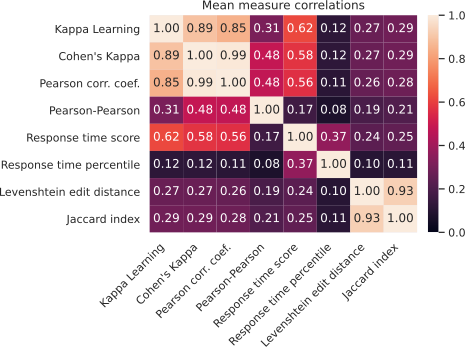
\includegraphics[width=0.7\linewidth]{figures/heatmap_mean_correlations}
	\end{center}
\end{frame}


\begin{frame}
	\frametitle{Amount of data required}
	\begin{center}
		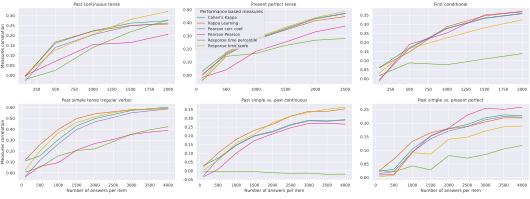
\includegraphics[width=1\linewidth]{figures/perf_jaccard_corrs}
	\end{center}
\end{frame}

\begin{frame}
	\frametitle{Difference among knowledge components}
	\begin{itemize}
		\item Correlations range from 0.06 to 0.67.
		\item The choice of knowledge component is more significant than the choice of measures.
		\begin{itemize}
			\item Rule-based components have higher correlations on average.
			\item Items for lower grades have higher correlations.
			\item Newly added items lower the correlations. 
		\end{itemize}
	\end{itemize}
\end{frame}

\begin{frame}
\frametitle{Message}
\begin{enumerate}
\item Performance-based similarity measures are data-hungry.
\bigskip
\item Results from one knowledge component may not generalize to others.
\end{enumerate}
\end{frame}

\begin{frame}[standout]
	\frametitle{}
	\begin{center}
		Thank you for your attention.
	\end{center}
	\vfill
	{
		\raggedright
		\footnotesize
		Experimental Evaluation of Similarity Measures for Educational Items\\
		J. Čechák, R. Pelánek
		
	}

\end{frame}


\end{document}
